\documentclass[conference]{IEEEtran}

%\usepackage{natbib}
\usepackage{multirow}
\usepackage{mathtools}
\usepackage{fixltx2e}
\usepackage{amssymb}
\usepackage{graphics}
\usepackage{balance}

\title{Vida artificial: Simulaci\'on de vida artificial y su impacto en el estudio de la biodiversidad }

% author names and affiliations

\author{\IEEEauthorblockN{David S\'anchez Alb\'an,   Natalia Mar\'in P\'erez}
\IEEEauthorblockA{Ingenier\'ia en Ciecias de la Computaci\'on\\
Instituto Tecnol\'ogico de Costa Rica\\
San Jos\'e, Costa Rica}

}
\begin{document} 

% make the title area
\maketitle


\begin{abstract}
%\boldmath
La vida y su interacci\'on con el ser humano siempre ha sido de gran inter\'es a la hora de realizar estudios en la materia. 
bla bla bla... 



\end{abstract}

\section{Introducci\'on}

Vida artificial fue definida por Chris Langton como `el estudio de sistemas hechos por el hombre que exhibe comportamientos caracter\'isticos de sistemas vivos provenientes de la naturaleza' \cite{JDOY01}, es un \'area de estudio bastante reciente que puede guiar las investigaciones cient\'ificas en la manera de extender la vida y crear nuevas formas de ella, incluyendo medicinas, internet, hardware que pude evolucionar y la proliferaci\'on de robots. \cite{PROB01}\\
Es por esto que se nos da la tarea de poder simular vida a trav\'es de la computaci\'on para crear vida y de esta manera entenderla. \cite{artificiallifeLevy}  \\
Para crear vida artificial que sea robusta por computadora, es necesario que esta pueda sobrevivir las fluctuaciones del ambiente y evolucionar tan libremente como su vida biol\'ogica. El software debe poder adaptarse con algoritmos de aprendizaje que permitan a los programas de computadora ganar experiencia, as\'i como programas que sean capaces de escribir otros programas de computadoras con un comportamiento de "b\'usqueda de metas" que permita a los programas funcionar en ambientes espec\'ificos. El software de computadora debe poder innovar y agregar en s\'i mismo la respuesta a sus "necesidades". El solucionar estos problemas es una de las metas principales en el estudio de vida artificial \cite{JDOY01}.\\
En el an\'alisis acerca de herramientas de vida artificial escrito por Steven Levy se explica el de un sistema desarrollado por el bi\'ologo Thomas Ray el cual plantea una herramienta llamada "Tierra". Una vez que el sistema fue finalizado, este pod\'ia cambiar su criterio por el cual se constitu\'ia un organismo apto, y cuando este se llenaba de organismos el ambiente evolutivo cambiaba tambi\'en; las criaturas digitales fueron forzadas a buscar respuestas novedosas cuando las circunstancias eran alteradas. Esto se lograba gracias a sistemas de "reconocimiento", ya que de los contrario habr\'ian mutaciones que no se llevar\'ian a cabo. El sistema est\'a buscando constantemente en hacer el c\'odigo eficiente, pero por otra parte la evoluci\'on se da al "explotar" entre s\'i, los organismos agregan el concepto del m\'as apto, una nueva adaptaci\'on que se da al transmitir los genes que puede contener un mecanismo espec\'ificio que no necesariamente est\'a presente en el ancestro. Tierra refleja comunidades ecol\'ogicas al simular un depredador el cual va a suprimir al competidor y lo excluye como uno de los competidores d\'ebiles impactando as\'i en la diversidad. \cite{STEV01} \\

Una vez que se entiende una forma de vida y su comportamiento es posible ayudar en c\'omo estos podr\'ian impactar el ecosistema en que vivimos y entender mejor de que manera los seres vivos impactan en el medio ambiente.



\section{Marco Te\'orico}

% En el doc que tengo en drive tengo bastanteeeee que poner aca 


A la hora de poder desarrollar, estudiar o crear vida artificial, se debe de tener un entendimiento de la vida en s\'i, donde las m\'ultiples \'areas de la academia han intentado definir, qu\'e es? Los fil\'osofos utilizan t\'erminos para discernir entre lo vivo y lo no-vivo, y son estas cualidades lo que hace a algo pertenecer al \'area de los entes vivos. \cite{lifeStanfordPhi} En el area de la biolog\'ia se utiliza la reproducci\'on y la supervivencia \cite{artificiallifeLevy} como capacidades necesarias con el fin de definir algo como vivo. 

La vida es considerada org\'anica, ya que esta surge naturalmente y es un concepto irremplazable del mundo natural, la cual es un \'area de estudio para los bi\'ologos y dem\'as \'areas de la ciencia y tecnol\'ogia. El concepto de vida ha sido estudiado por cientos de a\~nos, pero siempre existen conflictos a la hora poder definir una definici\'on concreta, por ejemplo: Arist\'oteles defini\'o la vida como la propiedad de un objeto de ser animado, Descartes como un mecanismo, el punto de vista de Kant como una organizaci\'on. \cite{lifeStanfordPhi} \\
Tambi\'en es importante entender lo que es la vida natural, la cual tiene las siguientes caracter\'isticas \cite{XUY01} :
\begin{itemize}
\item Crecimiento natural, evoluci\'on y no hecho por el hombre.
\item Reproducci\'on sexual, por ejemplo, humanos, otros animales y plantas
\item Basado en prote\'inas, sustancias org\'anicas.
\item Inteligencia y emociones, tales como el humano u otros animales
\end{itemize}

Pero qu\'e pasa cuando la biolog\'ia y las ciencias de la computaci\'on se mezclan, con esto surge la pregunta, ser\'a el poder computacional actual capaz de emular las cualidades necesarias para crear vida artificial? A esto se ha llamado vida `in-silico' \cite{artificiallifeLevy, lifeStanfordPhi} esto por el uso de los chips semiconductores necesarios para el uso de software. El uso de la vida in-silico se debe primariamente a la gran capacidad de procesamiento que poseen las computadoras para evaluar modelos complejos sobre vida artificial, a parte de poder ayudarnos a mejorar el concepto de vida artificial que tenemos. 

Parte de la teor\'ia que podria mostrar el flujo de la vida seria el uso de teor\'ia de automatas, para poder crear una visualizacion la cual satisfaga todas las opciones que sean necesarias para mostrar vida bajo una definicion especifica. Para esto se podria usar una Maquina de Estados Finitos (FSM) \cite{MARG01} la cual nos ayude a demostrar una serie de estados en la cual un organismo puede estar, pero, esto generar\'ia un FSM demasiado grande, el cual seria inmanejable para un ser humano, pero una computadora podria re-crear un ente sencillo, d\'igase de una bacteria o un insecto.  

En el a\~no 1982, el cient\'ifico Stephem Wolfram explor\'o y categoriz\'o los tipos de complejidad que mostraban los autómatas celulares unidimensionales, y se dieron cuenta que estos podr\'ian ser aplicados a fen\'omenos naturales como las conchas marinas y la naturaleza del crecimiento de las plantas. Tambi\'en, Norman Packard utiliz\'o los aut\'omatas celulares para simular el crecimiento de copos de nieve. \cite{VAD01} \\
Existen dos posiciones en vida artificial\cite{VAD01} :
\begin{itemize}
\item La posici\'on fuerte/dura que indica que "la vida es un proceso que se puede conseguir fuera de cualquier medio particular". (John Von Neumann). Como se indicaba anteriormente en el sistema Tierra donde la vida era sintetizada seg\'un Thomas Ray.
\item La posici\'on d\'ebil la cual niega la posibilidad de generar un "proceso de vida" fuera de una soluci\'on qu\'imica basada en el carbono, en cambio se opta por imitar procesos de vida para entender aspectos de fen\'omenos sencillos.
\end{itemize}


Un claro ejemplo del uso de vida artificial es el uso de modelos complejos con el fin de evaluar los resultados y obtener una simulaci\'on para satisfacer las pruebas necesarias, estos modelos pueden ayudarnos a explicar un comportamiento espec\'ifico. Tomemos el caso de las abejas arboricuas Apis mellifera, las cuales recolectan polen con el fin de transformarlo en miel y mantener la supervivencia de su colonia, estas poseen un comportamiento interesante a la hora de escojer las flores adecuadas, debido a que solamente estas proporcionan el polem adecuado para producir su preciada miel. \cite{ZOE01} El uso de vida artificial es imprecidible para poder crear un ambiente digital en el cual las abejas virtuales o agentes puedan interactuar con su medio, asimismo se pueden evaluar ambientes mas complejos y reducir el trabajo de campo. 

Estas tecnolog\'ias permiten a los ciencit\'ificos poder crear mo\'delos de organismos, o en el caso del estudio de enjambres de abejas, los cuales al ser un conjunto de abejas se les considera un superorganismo, ya que entre todos los organismos individuales se realizan operaciones complejas.\cite{TMRT01} La idea principal detr\'as del estudio era poder ver la coperaci\'on entre dos enjambres, los cuales se comportan de manera aleatoria y al encontrarse con otro, cada organismo interact\'ua individualmente con el otro. Esta investigaci\'on funciono para poder probar que las interacciones aleatorias entre abejas son dependientes del tama\~no de cada conglomerado.  

Adem\'as, existe un estudio alrededor de las hormigas  Leptothorax tuberointerruptus,\cite{LP01}, las cuales formaron parte esencial a la hora de realizar la investigaci\'on para proponer un modelo consistente y continuo el cual permite controlar un algoritmo el cual cree arquitecturas nuevas en sus nidos, donde dicha arquitectura afecta las relaciones f\'isicas que existen entre las hormigas, piedras y feromonas en el ambiente.
En dicho estudio se realizan pruebas con bastantes variables las cuales son afectadas por dos tipos de hormigas, las hormigas internas y las externas, las cuales forman parte de un una colonia de hormigas y son internas si est\'an dentro del \"nido\" o externas si est\'n fuera de \'el. Luego existe un conjunto de piedras las cuales, las hormigas pueden mover para ir formando la arquitectura del nido, estas piedras van formando el nido conforme el tiempo avanza. Asimismo existe una variante importante la cual se basa en el concepto de feromonas, estas feromonas afectan el comportamiento y movimiento de las hormigas.\cite{LP01}
Luego de que las hormigas forman el nido estas forman patrones interesantes, pero los autores explican que dentro de las pruebas estos encontraron que casi siempre los nidos tendi\'an a ser circulares y formar un conglomerado de hormigas internas. 

Luego no solamente se realizan los estudios alrededor de un solo organismo, en este caso tenemos que se evalu\'a como los organismos se comportan en un ambiente abierto y se evalu\'an sus movimientos ya que la cantidad de interacciones sociales es proporcional a la cantidad de individuos en el ambiente, asi se ven las interacciones que existen en una poblaci\'on de organismos. \cite{ASTK01, PMLC01}
Los individuos de la poblaci\'ion son manejadas por un algoritmo probabil\'ístico jer\'arquico el cual sirve para poder detectar las se\~nales externas que puedan afectar el patron de movimiento, ya sea un depredador o una fuente de calor. 
Para esto se evaularon 3 poblaciones:
\begin{itemize}
\item Mosquitos movimiento es generado por factores externos y no perciben a otros mosquitos.
\item Aves, solamente pueden moverse hacia el frente y tienen un rango de visi\'on limitado, no perciben otras aves.
\item Peces solamente ven a sus vecinos m\'as cercanos y se mueven con ellos y no pueden ver m\'as all\'a del rango de visibilidad que poseen.
\end{itemize}
Al finalizar las representaciones, los mosquitos se mostraban estar calmados por s\'i solos y no presentaban ningun patron especifico mas que la aleatoriedad de sus movimientos. Mientras que las aves y los peces forman patrones y se ven m\'as unidos en las visualizaciones. \cite{ASTK01}

No solamente los estudios se centran en el analisis de vida a nivel macroscopico, sino que tambien hay estudio para la vida microscopica, por ejemplo: simular una celula con el fin de poder estudiar tres apectos clave
\cite{shinji01} :
\begin{itemize}
\item Expresar geneticamente el m\'odelo de una celula encapsulado en un liposoma para poder habilitar sintesis de proteinas membrana. 
\item Una estructura con multiples roles los cuales esten dise\~nados para la nanoestructura del DNA en la membrana ceuluar. 
\item Una membrana de peptidos para poder detectar superficies.
\end{itemize}


\section{Simulaci\'ones y su impacto en el ecosistema}

En los estudios mencionados previamente se observa un gran inter\’es por encontrar m\'as acerca de, que es la vida? Nuestro m\'etodo de poder mostrar qu\’e significa el concepto para nosotros r\'adica en com\’o podemos demostrar nuestro conocimiento de la vida, plasmando en un mundo computacional. 
Tomemos el ejemplo de las hormigas y las abejas, estamos intentando crear organismos virtuales los cuales tienen una interacci\'on limitada con su medio ambiente el cual no cambia ni tampoco muestra amenazas potenciales para los mismos, ya que ninguna de estas fue programada para dichos entes virtuales. Pero aparte no es de sorprenderse de que utilicemos estos para poder simular y entender a los organismos a nuestro alrededor en base a simulaciones muy b\’asicas. Donde dichas simulaciones se basan en encontrar los comportamientos clave de cada una de estas especies, por ejemplo tenemos que para el paper relacionado con hormigas este intenta buscar los patrones por los cuales estas construyen sus impresionantes arquitecturas en sus hormigueros, para el caso del estudio mostrado, tienen su base hormigas, piedras y feromonas, donde las feromonas forman parte vital para controlar c\’omo las hormigas se comportan y forman el nido. 
Asimismo est\’an las abejas productoras de miel, por las cuales tienen un aprendizaje con respecto a las flores que son potenciales proveedores de polen para producir su preciado producto, la miel. 
Si se analiza a detalle ambas investigaciones buscan demostrar parte del comportamiento vital para el funcionamiento de estos organismos, ya sea las hormigas construyendo un hormiguero para proteger su colonia o abejas para poder producir miel, ambas se caracterizan por intentar demostrar como los entes vivos se manifiestan en su ambiente, y que los hace a estos vivos. 

\section{Posible contribuci\'on de Costa Rica en vida artificial}

\subsection{Estudio de abejas por parte de la Universidad Nacional}
Existen muchos \'ambitos en los que Costa Rica podr\'ia ser part\'icipe a nivel del estudio para estudios futuros en vida artificial. La Universidad Nacional tiene un instituto especializado en el estudio de las abejas tropicales para el desarrollo de una apicultura y meliponicultura sostenible en Costa Rica y Centroam\'erica. \cite{CINAT} . En el CINAT se encuentran una serie de publicaciones y estudios que se han realizado, por ejemplo en el paper publicado en el 2006 por S.E Berrocal se documenta el comportamiento de abejas en un ambiente controlados, Se busc\'o una posici\'on lateral del nido para colectar cargas de polen de las abejas mediante succionadores, este nido se monitoreaba cada 15 minutos durante las 3 horas de la recolecta. Seg\'un se puede ver en la figura ~\ref{fig:muestra} a partir de las 11:15am disminuyeron las abejas y las que llegaban trajeron material resinoso, del cual solo se pudo extraer dos muestras de polen, hay cierta certeza que la lluvia pudo haber impactado en su comportamiento.\cite{APICOLA}
\begin{figure}[ht]
%\centering
  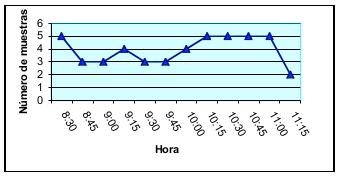
\includegraphics[width=9cm,height=5cm]{img/muestras.jpg}
  \caption{N\'umero de muestras por intervalo de 15 minutos. \cite{APICOLA}}
  \label{fig:muestra}
\end{figure}

\subsection{Simulaci\'on de Abejas Artificiales}
Para la simulaci\'on de abejas artificiales es necesario entender el comportamiento biol\'ogico de las abejas, se tiene que las abejas de miel escanean su objetivo de manera serial que son m\'as r\'apidos pero que se vuelven considerablemente lentos cuando los distractores que deben tambi\'en ser procesados por el sistema visual est\'an presentes como se puede mostrar en la figura ~\ref{fig:serial_honey} . As\'i que se tiene informaci\'on finita a nivel del procesamiento visual pero hay una amplia variedad de posibles ambientes naturales. El modelo que se establece en el documento es b\'asicamente basado en la el escaneo de la visi\'on, pero no se considera el olfato que utiliza normalmente las abejas para encontrar las flores(Streinzer, Paulus et al. 2009) \cite{ZOE01}. \\
Las abejas lo que hacen es buscar un mundo con una matriz de sus objetivos y las flores "distractoras", se determinan las distribuciones florales en las cuales cada mecanismo de escaneo visual podr\'ia ser m\'as efectivos en escenarios del mundo real. Estas simulaciones permiten interpretar que factores influencias adem\'as del c\'omo y el porqu\'e las abejas toman decisiones, adem\'as de los beneficios que recibir\'ia a nivel de la colonia como factores relevantes para el \'exito reproductivo.\cite{ZOE01} \\

\begin{figure}[ht]
%\centering
  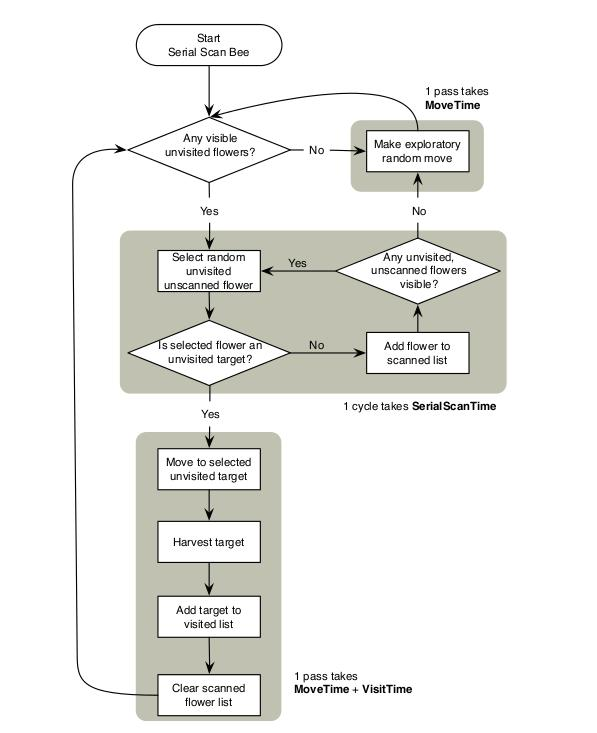
\includegraphics[width=8cm,height=8cm]{img/serial_honey.jpg}
  \caption{El flujo de escaneo serial de una abeja de miel \cite{ZOE01}}
  \label{fig:serial_honey}
\end{figure}


\subsection{Simulaciones y medio ambiente}
Como se demuestra en el paper de Abejas Artificiales (tambi\'en conocidas como A-bees) se demuestra como las abejas de miel pueden ser m\'as efectivas en ambientes donde los objetivos no son segregados junto con distractores, por otra parte este trabajo fue ejecutado con entradas de comportamiento conocido en abejas en ambiente templado pero todav\'ia es necesario compararlo con abejas tropicales.
Tambi\'en se puede sugerir que el cambio de clima puede afectar en la disponibilidad de la flor (a nivel de tiempo-espacio) y de los mismos agentes polinizadores debido a la capacidad visual de las abejas. Como tambi\'en se detalla en la observaci\'on de S.E Berrocal (Universidad Nacional) hubo momentos, posiblemente por la lluvia en las que las abejas no polinizaban, el poder entender m\'as fondo estas especies podr\'ia proporcionar informaci\'on importante para el futuro de los manejo de recursos y a la actividad ap\'icola. 


\section{Trabajo relacionado}

Open worm es un estudio y/o proyecto el cual esta intentado re-crear una lombriz utilizando la vida artificial simulado por computadores.  Al simular las mil c\'elulas de la lombriz Caenorhabditis elegans (C. elegans) se lograr\'a entender comportamientos simples y complejos lo cual satisface lo suficiente para poder realizar un estudio compresivo al respecto, esta posee comportamientos clave como: alimentaci\'on, reproducci\'on, evitar depredadores, entre otras caracter\'isticas. \cite{openworm} Todas estas caracteristicas son vitales para poder entender el concepto filos\'ofico de qu\'e es la vida y cu\'ales son sus componentes b\'asicos para el estudio al respecto. \\
Aunque ha sido estudiado profundamente, a\'un hace falta tener un mayor entendimiento de los principios de su biolog\'ia.
Una vez que se logre la meta se espera que esto ayudar\'a a la creaci\'on de otras criaturas virtuales que sean igual de precisas.
Aparte de ser una herramienta sumamente importante, Open worm... % MUERO, http://docs.openworm.org/en/0.9/Community/github/, seguir ahi. 

\section{Conclusi\'on}

Existen estudios... es interesante porque... los apredido fue...

\nocite{*}

\bibliographystyle{IEEEtranS} % ordena por nombre de autor
\bibliography{vida_artificial}
\end{document}
